% Copyright (c) 2010 Jérémie DECOCK (http://www.jdhp.org)

% This document is provided under the terms of the "Creative Commons BY-SA" license.
% For more details, read "legalcode.html" enclosed file or "http://creativecommons.org/licenses/by-sa/2.0/fr/" web page.

%\documentclass[draft]{beamer}
\documentclass{beamer}

%%%%%%%%%%%%%%%%%%%%%%%%%%%%%%%%%%%%%%%%%%%%%%%%%%%%%%%%%%%%%%%%%%%%%%%%%%%%%%%%

%\documentclass[handout]{beamer}
%
%\usepackage{pgfpages}
%
%\pgfpagesdeclarelayout{3 on 1 with notes}
%{
%  \edef\pgfpageoptionheight{\the\paperheight}
%  \edef\pgfpageoptionwidth{\the\paperwidth}
%  \edef\pgfpageoptionborder{0pt}
%}
%{
%  \pgfpagesphysicalpageoptions
%  {
%    logical pages=3,
%    physical height=\pgfpageoptionheight,
%    physical width=\pgfpageoptionwidth
%  }
%  \pgfpageslogicalpageoptions{1}
%  {
%    border shrink=\pgfpageoptionborder,
%    resized width=.5\pgfphysicalwidth,
%    resized height=.33\pgfphysicalheight,
%    center=\pgfpoint{.25\pgfphysicalwidth}{.825\pgfphysicalheight}
%  }
%  \pgfpageslogicalpageoptions{2}
%  {
%    border shrink=\pgfpageoptionborder,
%    resized width=.5\pgfphysicalwidth,
%    resized height=.33\pgfphysicalheight,
%    center=\pgfpoint{.25\pgfphysicalwidth}{.495\pgfphysicalheight}
%  }
%  \pgfpageslogicalpageoptions{3}
%  {
%    border shrink=\pgfpageoptionborder,
%    resized width=.5\pgfphysicalwidth,
%    resized height=.33\pgfphysicalheight,
%    center=\pgfpoint{.25\pgfphysicalwidth}{.165\pgfphysicalheight}
%  }
%}
%
%\pgfpagesuselayout{3 on 1 with notes}[a4paper,border shrink=5mm]

%%%%%%%%%%%%%%%%%%%%%%%%%%%%%%%%%%%%%%%%%%%%%%%%%%%%%%%%%%%%%%%%%%%%%%%%%%%%%%%%

\usepackage[utf8]{inputenc}
\usepackage[frenchb]{babel}

% Theme
% default, Dresden, Darmstadt, Frankfurt, Singapore
%\usetheme[⟨options⟩]{default}
%\usecolortheme[⟨options⟩]{default}
%\usefonttheme[⟨options⟩]{default}
%\useinnertheme[⟨options⟩]{default}
%\useoutertheme[⟨options⟩]{default}
\usetheme[compress]{Dresden}

\title{Le droit du logiciel}
\subtitle{Droit d'auteur et brevet}

% \author[⟨short author names⟩]{⟨author names⟩}
% The names should be separated using the command \and.
\author[Decock]{Jérémie~\bsc{Decock}}

\institute{UPMC}
\date{25 octobre 2010}

% \subject{⟨text⟩}
% Enters the ⟨text⟩ as the subject text in the pdf document info.
% It currently has no other effect.
\subject{Droit d'auteur et brevet}

% \keywords{⟨text⟩}
% Enters the ⟨text⟩ as keywords in the pdf document info.
% It currently has no other effect. 
\keywords{droit d'auteur, brevets, logiciels}

\AtBeginSection[] {
    %\begin{frame}<beamer>{Plan}
    \begin{frame}<beamer>
        \tableofcontents[currentsection,currentsubsection]
    \end{frame}
}

\AtBeginSubsection[] {
    %\begin{frame}<beamer>{Plan}
    \begin{frame}<beamer>
        \tableofcontents[currentsection,currentsubsection]
    \end{frame}
}

\begin{document}

%%%%%%%%%%%%%%%%%%%%%%%%%%%%%%%%%%%%%%%%%%%%%%%%%%%%%%%%%%%%%%%%%%%%%%%%%%%%%%%

\begin{frame}
    \titlepage
\end{frame}

%%%%%%%%%%%%%%%%%%%%%%%%%%%%%%%%%%%%%%%%%%%%%%%%%%%%%%%%%%%%%%%%%%%%%%%%%%%%%%%

\begin{frame}{Plan}
    \tableofcontents
\end{frame}

%%%%%%%%%%%%%%%%%%%%%%%%%%%%%%%%%%%%%%%%%%%%%%%%%%%%%%%%%%%%%%%%%%%%%%%%%%%%%%%

\section{Le droit d'auteur}

\subsection{Pourquoi les logiciels sont-ils protégés par le droit d’auteur~?}

\begin{frame}{Le contexte}
    Le statut du logiciel au début de l'industrie informatique
    \begin{itemize}
        \item une activité industrielle
        \item un service
    \end{itemize}
    \begin{block}{Apparition du progiciel dans les années 70}
        \og{}Produit logiciel commercialisé de façon autonome et standard,
        ce qui suppose un certain degré de portabilité\fg{}
        (Jean-Benoît~\bsc{Zimmermann})
    \end{block}
    ~\\
    Quel statut pour ce bien marchand d'un genre nouveau~?
    \begin{itemize}
        \item brevet d'invention~?
        \item droit d'auteur~?
        \item un cadre juridique spécifique~?
    \end{itemize}
\end{frame}

\begin{frame}{Les textes adoptés}
    \begin{block}{Loi du 3 juillet 1985 (France)}
        Les logiciels \og{}originaux\fg{} sont protégés par le droit d'auteur
    \end{block}
    \begin{block}{Directive 91/250/CEE du Conseil (14 mai 1991)}
        Les logiciels sont protégés par le droit d'auteur sur le territoire européen (art.~1)
    \end{block}
    \begin{block}{Loi du 10 mai 1994 (France)}
        Harmonisation avec la directive européenne du 14 mai 1991
    \end{block}
    \begin{block}{Traité de l’OMPI sur le droit d’auteur (20 décembre 1996)}
        Les logiciels sont protégés par le droit d'auteur dans tous les pays signataires (art.~4)
    \end{block}
\end{frame}

\begin{frame}{La solution retenue (en France et en Europe)}
    En France et en Europe~:
    \begin{itemize}
        \item les logiciels sont protégés par le droit d'auteur (CPI~art.~L112-2 et Directive 91/250/CEE)
        \item les logiciels \emph{en tant que tels} ne peuvent pas être brevetés (CPI~art.~L611-10 et CBE~2000~art.~52)
    \end{itemize}
\end{frame}

%%%%%%%%%%%%%%%%%%%%%%%%%%%%%%%%%%%%%%%

\subsection{Le droit d’auteur et les logiciels (en France)}

\begin{frame}{Les droits moraux et les droits patrimoniaux}
    \begin{block}{Le droit d’auteur}
        \emph{Code le la Propriété Intellectuelle} (\emph{CPI})
    \end{block}
    ~\\
    Droits moraux (appartiennent à l'auteur)~:
    \begin{itemize}
        \item respect du nom (CPI~art.~L121-1)
        \item libre choix de la divulgation de l'œuvre (CPI~art.~L121-2)
    \end{itemize}
    ~\\
    Droits patrimoniaux (appartiennent aux ayants droit)~:
    \begin{itemize}
        \item droit de reproduction de l'œuvre (CPI~art.~L122-1 )
        \item droit de représentation de l'œuvre (CPI~art.~L122-1 )
    \end{itemize}
\end{frame}

\begin{frame}{Les droits moraux et les droits patrimoniaux}
    Les droits moraux~:
    \begin{itemize}
        \item sont perpétuels, inaliénables et imprescriptibles (CPI~art.~L121-1)
        \item sont transmissibles aux héritiers après la mort de l'auteur (CPI~art.~L121-1)
    \end{itemize}
    ~\\
    Les droits patrimoniaux~:
    \begin{itemize}
        \item sont cessibles à titre gratuit ou onéreux (CPI~art.~122-7)
    \end{itemize}
    ~\\
    Droits moraux suspendus dans le cas du logiciel~:
    \begin{itemize}
        \item droit de repentir (CPI~art.~L121-7)
        \item droit à l'intégrité (CPI~art.~L121-7)
    \end{itemize}
\end{frame}

\begin{frame}{Les titulaires du droit d’auteur}
    \og{}La qualité d'auteur appartient, sauf preuve contraire, à celui ou
    à ceux sous le nom de qui l'œuvre est divulguée.\fg{} (CPI~art.~L113-1)\\
    ~\\
    Cas particuliers~:
    \begin{itemize}
        \item logiciel créé par plusieurs personnes physiques (\emph{œuvre
              de collaboration}) (CPI~art.~L113-3)
        \item logiciel créé par plusieurs personnes physiques sous la
              direction d'une personne physique ou morale qui a pris
              l'initiative de le créer (\emph{œuvre collective})
              (CPI~art.~L113-5)
        \item logiciel développé dans une entreprise (CPI~art.~L113-9 et
              L121-1)
    \end{itemize}
\end{frame}

\begin{frame}{Les exceptions au droit d'auteur}
    Les exceptions au droit d'auteur (CPI~art.L122-5)~:
    \begin{itemize}
        \item copie privée
        \item représentation dans le cercle familial
        \item etc.
    \end{itemize}
    ~\\
    Les exceptions particulières pour les logiciels (CPI~art.L122-6-1)~:
    \begin{itemize}
        \item analyse du fonctionnement du logiciel
        \item correction d'erreurs de conception
        \item décompilation motivée par un souci d'interopérabilité
        \item etc.
    \end{itemize}
\end{frame}

\begin{frame}{Les éléments protégés}
    \begin{itemize}
        \item l'architecture du programme
        \item le code source
        \item le code objet (code source compilé)
        \item les éléments multimédia incorporés (son, texte, image, vidéo)
        \item les écrans et modalités d'interactivité (s'ils sont originaux)
        \item le matériel de conception préparatoire~: les ébauches,
              les maquettes, les dossiers d'analyses fonctionnelles,
              la documentation intégrée au logiciel, les prototypes
    \end{itemize}
\end{frame}

\begin{frame}{Les éléments non protégés}
    \begin{itemize}
        \item les fonctionnalités
        \item les algorithmes
        \item les interfaces
        \item les langages de programmation
    \end{itemize}
\end{frame}

\begin{frame}{Les modalités de protection}
    % Aucune modalité n'est requise
    \og{}L'œuvre est réputée créée, indépendamment de toute divulgation
    publique, du seul fait de la réalisation, même inachevée, de
    la conception de l'auteur.\fg{} (CPI~art.~L111-2)\\
    ~\\
    Recommandations~:
    \begin{itemize}
        \item la mention copyright pour les pays n'adhérant pas à la Convention de Berne
        \item déposer l'œuvre (constituer une preuve d'antériorité)
    \end{itemize}
    ~\\
    Le dépôt~:
    \begin{itemize}
        \item \emph{APP}
        \item \emph{INPI}~: enveloppe Soleau (papier seulement)
        \item huissier de justice
    \end{itemize}
\end{frame}

%%%%%%%%%%%%%%%%%%%%%%%%%%%%%%%%%%%%%%%%%%%%%%%%%%%%%%%%%%%%%%%%%%%%%%%%%%%%%%%

\section{Les brevets d'invention}

\subsection{Les brevets}

\begin{frame}{Les brevets~: objectifs}
    Protéger une invention
    \begin{itemize}
        \item confère à son propriétaire un droit exclusif d’exploitation
              sur une invention
        \item valable 20 ans
        \item valable uniquement sur un territoire déterminé (un pays unique
              ou un groupe de pays)
    \end{itemize}
    ~\\
    Favoriser la recherche et l'innovation (contreparties)
    \begin{itemize}
        \item l'invention doit être divulguée au public
        \item l'invention tombe dans le domaine public à l'issue de la
              période de protection
    \end{itemize}
\end{frame}

\begin{frame}{La portée des brevets}
    La portée des brevets~:
    \begin{itemize}
        \item brevets nationaux~: un seul pays
        \item brevets régionaux~: plusieurs pays
    \end{itemize}
    ~\\
    Les organismes gérant les brevets~:
    \begin{itemize}
        \item France~: \emph{INPI}
        \item Europe~: \emph{OEB} (\emph{EPO})
        \item États Unis~: \emph{USPTO}
        \item ONU~: \emph{OMPI} (\emph{WIPO})
    \end{itemize}
\end{frame}

\begin{frame}{Les critères de brevetabilité (en France)}
    \begin{itemize}
        \item l’invention doit être nouvelle (CPI~art.~L611-11)
        \item l’invention doit impliquer une activité inventive
              (CPI~art.~L611-15)
        \item l’invention doit être susceptible d’application industrielle
              (CPI~art.~L611-15)
    \end{itemize}
\end{frame}

\begin{frame}{Les travaux non brevetables (en France)}
    En raison de leur caractère abstrait (CPI~art.~L611-10)~:
    \begin{itemize}
        \item les découvertes, théories scientifiques et méthodes
              mathématiques
        \item les plans, principes et méthodes dans l’exercice d’activités
              intellectuelles, ainsi que les \emph{programmes d’ordinateur}
        \item les présentations d’informations
        \item les créations esthétiques
    \end{itemize}
    ~\\
    Pour des raisons éthiques (CPI~art.~L611-17 à L611-19)~:
    \begin{itemize}
        \item les inventions contraires à l’ordre public et aux bonnes mœurs
        \item les espèces animales ou végétales
        \item les séquences totales ou partielles d'un gène en tant que telles
        \item les méthodes de traitement chirurgical ou thérapeutique du
              corps humain ou animal et les méthodes de diagnostic
    \end{itemize}
\end{frame}

\begin{frame}{Classification internationale des brevets (CIB)}
    \begin{block}{Qu'est-ce que c'est~?}
        Un système hiérarchique permettant de classifier les brevets
    \end{block}
    ~\\
    \begin{block}{Objectif}
        Faciliter les recherches sur les brevets connus à l'échelle mondiale
    \end{block}
\end{frame}

%%%%%%%%%%%%%%%%%%%%%%%%%%%%%%%%%%%%%%%

\subsection{Les brevets logiciels}

\begin{frame}{La situation actuelle en Europe (rappel)}
    Ce que disent les textes en France et en Europe~:
    \begin{itemize}
        \item les logiciels sont protégés par le droit d'auteur (CPI~art.~L112-2 et Directive 91/250/CEE)
        \item les logiciels \emph{en tant que tels} ne peuvent pas être brevetés (CPI~art.~L611-10 et CBE~2000~art.~52)
    \end{itemize}
    ~\\
    La situation réelle (source \emph{ffii.org})~:
    \begin{itemize}
        \item l'OEB accorde chaque année des dizaines de milliers de brevets logiciels
        \item certains sont abstraits et détachés de tout procédé technique
        \item d'autres sont \og{}triviaux\fg{} (brevet \emph{EP 394160} sur la barre de progression)
    \end{itemize}
\end{frame}

\begin{frame}{La situation actuelle dans le reste du monde}
    Certains pays autorisent expressément les brevets logiciels~:
    \begin{itemize}
        \item les États Unis
        \item le Japon
        \item l'Australie
        \item etc.
    \end{itemize}
\end{frame}

\begin{frame}{Les différents points de vue}{Les défenseurs des brevets logiciels}
    \begin{block}{Leur principal reproche}
        Le droit d'auteur ne protège que la forme et non le concept créatif
        (algorithmes et fonctionnalités)
    \end{block}
    \begin{block}{Ce qu'ils souhaitent}
        Protéger le concept inventif des logiciels, et non plus seulement sa
        mise en forme, ce que permettraient les brevets logiciels
    \end{block}
\end{frame}

\begin{frame}{Les différents points de vue}{Les opposants aux brevets logiciels}
    \begin{block}{Leur position}
        Les brevets logiciels risquent de créer un déséquilibre en faveur
        des grands éditeurs et de renforcer les monopoles au détriment des
        petits éditeurs et des clients
    \end{block}
    \begin{block}{Leur argument}
        Les petites entreprises et les développeurs indépendants n'auront
        pas les moyens financiers de s'engager dans la course aux brevets
    \end{block}
\end{frame}

\begin{frame}{Les différents points de vue}{Les opposants aux brevets logiciels}
    \begin{block}{Ce qu'ils affirment}
        Le droit d'auteur appliqué aux logiciels ne bloque pas l'innovation
    \end{block}
    \begin{block}{Ce qu'ils dénoncent}
        Les dérives que l'on peut observer dans les pays appliquant les
        brevets logiciels (brevets portant sur des idées triviales ou sur
        des concepts)
    \end{block}
\end{frame}

\begin{frame}{Les brevets triviaux}{Quelques exemples (source \emph{ffii.org})}
    \begin{columns}[c]
        \begin{column}{.50\linewidth}
            % contenu
            \begin{center}
                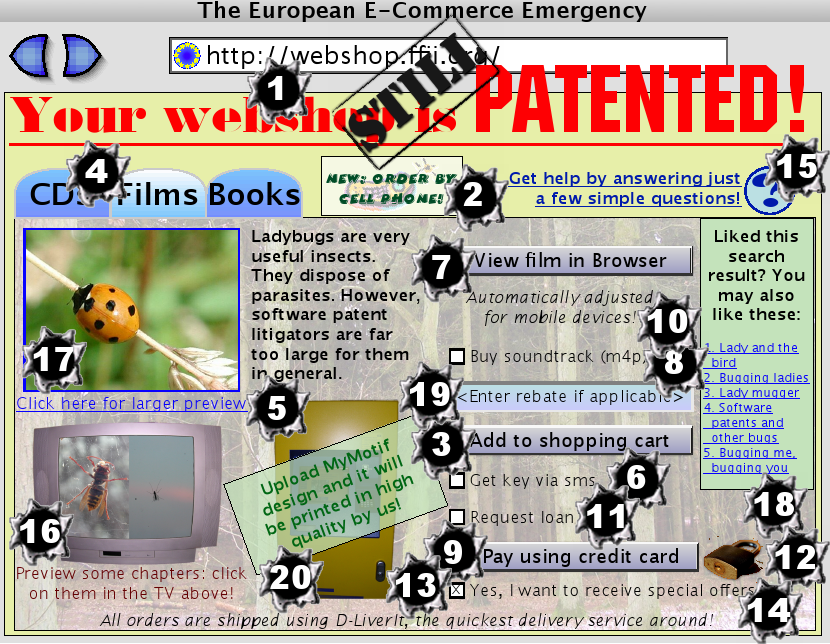
\includegraphics[width=.99\linewidth]{images/webshop}
            \end{center}
        \end{column}
        \begin{column}{.50\linewidth}
            % contenu
            \begin{tiny}
                \begin{enumerate}
                    \item  Webshop: Selling things over a network using a server, client and payment processor, or using a client and a server - EP803105, EP738446 and EP1016014
                    \item Order by cell phone: Selling over a mobile phone network - EP1090494
                    \item Shopping cart: Electronic shopping cart - EP807891
                    \item CDs Films Books: Tabbed palettes and restrict search - EP689133 and EP1131752
                    \item Picture link: Preview window - EP537100
                    \item Get key via sms: Sending key to decrypt bought data via mobile phone network - EP1374189
                    \item View film: Video streaming ("segmented video on-demand") - EP633694
                    \item Copy protection: Encrypt file so it can only be played on authorised devices - EP1072143
                    \item Credit card: Pay with credit card on the Internet - EP779587
                    %\item Adapt pages: Generate different web page depending on detected device - EP1320972
                    %\item Request loan: Automated loan application - EP715740
                    %\item Secure card payment: Secure online credit/debit card payment with PIN code - EP1218865
                    %\item Send oers: Send oers in response to request - EP986016
                    %\item Delivery: Ship items to the correct pick-up point of the used delivery service - EP1181655
                    %\item Support system: Support system based on answers to questions - EP915422
                    %\item Preview chapters: Use of TV as metaphor for selecting different video fragments - EP670652
                    %\item Image: Reduce page loading time by automatically reducing image quality - EP992922
                    %\item Related results: Show related results if customer likes the current ones - EP628919
                    %\item Rebate code: Allow rebate codes to be entered by customers - EP929874
                    %\item Web-to-Print: Generation of prepress formats or printouts from low resolution templates via the Internet - EP852359 and EP1169848
                \end{enumerate}
            \end{tiny}
        \end{column}
    \end{columns}

\end{frame}

\begin{frame}{Une tentative de légalisation des brevets logiciels en Europe}
    Propositions de directives au niveau européen~:
    \begin{itemize}
        \item vote (en première lecture) au Parlement Européen le 24 septembre
              2003 à Strasbourg
        \item adoption (en première lecture) en Conseil des Ministres le
              7 mars 2005 de l'accord politique sur les brevets logiciels
              du 18 mai 2004 à Bruxelles
        \item rejet par le parlement lors du vote (en deuxième lecture)
              le 6 juillet 2005 à Strasbourg
    \end{itemize}
    ~\\
    \begin{block}{Mais\dots}
        Le traité de Lisbonne tente de redistribuer les cartes en créant
        une nouvelle juridiction de brevet européenne
    \end{block}
\end{frame}

\begin{frame}{Conclusion}
    \begin{block}{Les brevets}
        Ils permettent de stimuler les innovations industrielles
        en protégeant les procédés techniques tout en les ouvrant à la
        concurrence
    \end{block}
    ~\\
    \begin{block}{Les brevets logiciels}
        Le système du droit d'auteur semble plus adapté car ce sont des
        œuvres de l'esprit à mi-chemin entre les œuvres littéraires et
        les démonstrations mathématiques
    \end{block}
    ~\\
    \begin{block}{Le problème en Europe}
        Le flou entretenu par l'OEB qui accorde des brevets allant à
        l'encontre des textes en vigueurs
    \end{block}
\end{frame}

%%%%%%%%%%%%%%%%%%%%%%%%%%%%%%%%%%%%%%%%%%%%%%%%%%%%%%%%%%%%%%%%%%%%%%%%%%%%%%%

\appendix

\section*{References}

\begin{frame}[allowframebreaks]{Sources}
    \begin{itemize}
        \item IRPI : \url{http://www.irpi.ccip.fr}
        \item INPI : \url{http://www.inpi.fr}
        \item CBE 1973 art. 52~: \url{http://www.epo.org/patents/law/legal-texts/html/epc/1973/f/ar52.html}
        \item CBE 2000 art. 52~: \url{http://www.epo.org/patents/law/legal-texts/html/epc/2000/f/ar52.html}
        \item Directive 91/250/CEE du Conseil (14 mai 1991)~: \url{http://eur-lex.europa.eu/Notice.do?val=172880:cs&lang=fr&list=207460:cs,172880:cs,&pos=2&page=1&nbl=2&pgs=10&hwords=auteur~&checktexte=checkbox&visu=}
        \item Traité de l’OMPI sur le droit d’auteur (1996)~: \url{http://www.wipo.int/treaties/fr/ip/wct/trtdocs_wo033.html}
        \item L'APP~: \url{http://app.legalis.net}
        \item Legifrance~: \url{http://www.legifrance.gouv.fr}
        \item Wikipedia~: \url{http://fr.wikipedia.org}
        \item OEB~: \url{http://www.epo.org}
        \item APRIL~: \url{http://www.april.org/groupes/brevets/}
        \item nosoftwarepatents.com~: \url{www.nosoftwarepatents.com}
        \item endsoftwarepatents.org~: \url{http://endsoftpatents.org}
        \item AFUL~: \url{http://www.aful.org}
        \item brevets-logiciels.info~: \url{http://brevets-logiciels.info}
        \item FFII~: \url{http://eupat.ffii.org}
        \item Pierre Breese~: \url{http://www.breese.fr}
    \end{itemize}
\end{frame}

\begin{frame}
    \begin{center}
        \href{http://creativecommons.org/licenses/by-sa/2.0/fr/}{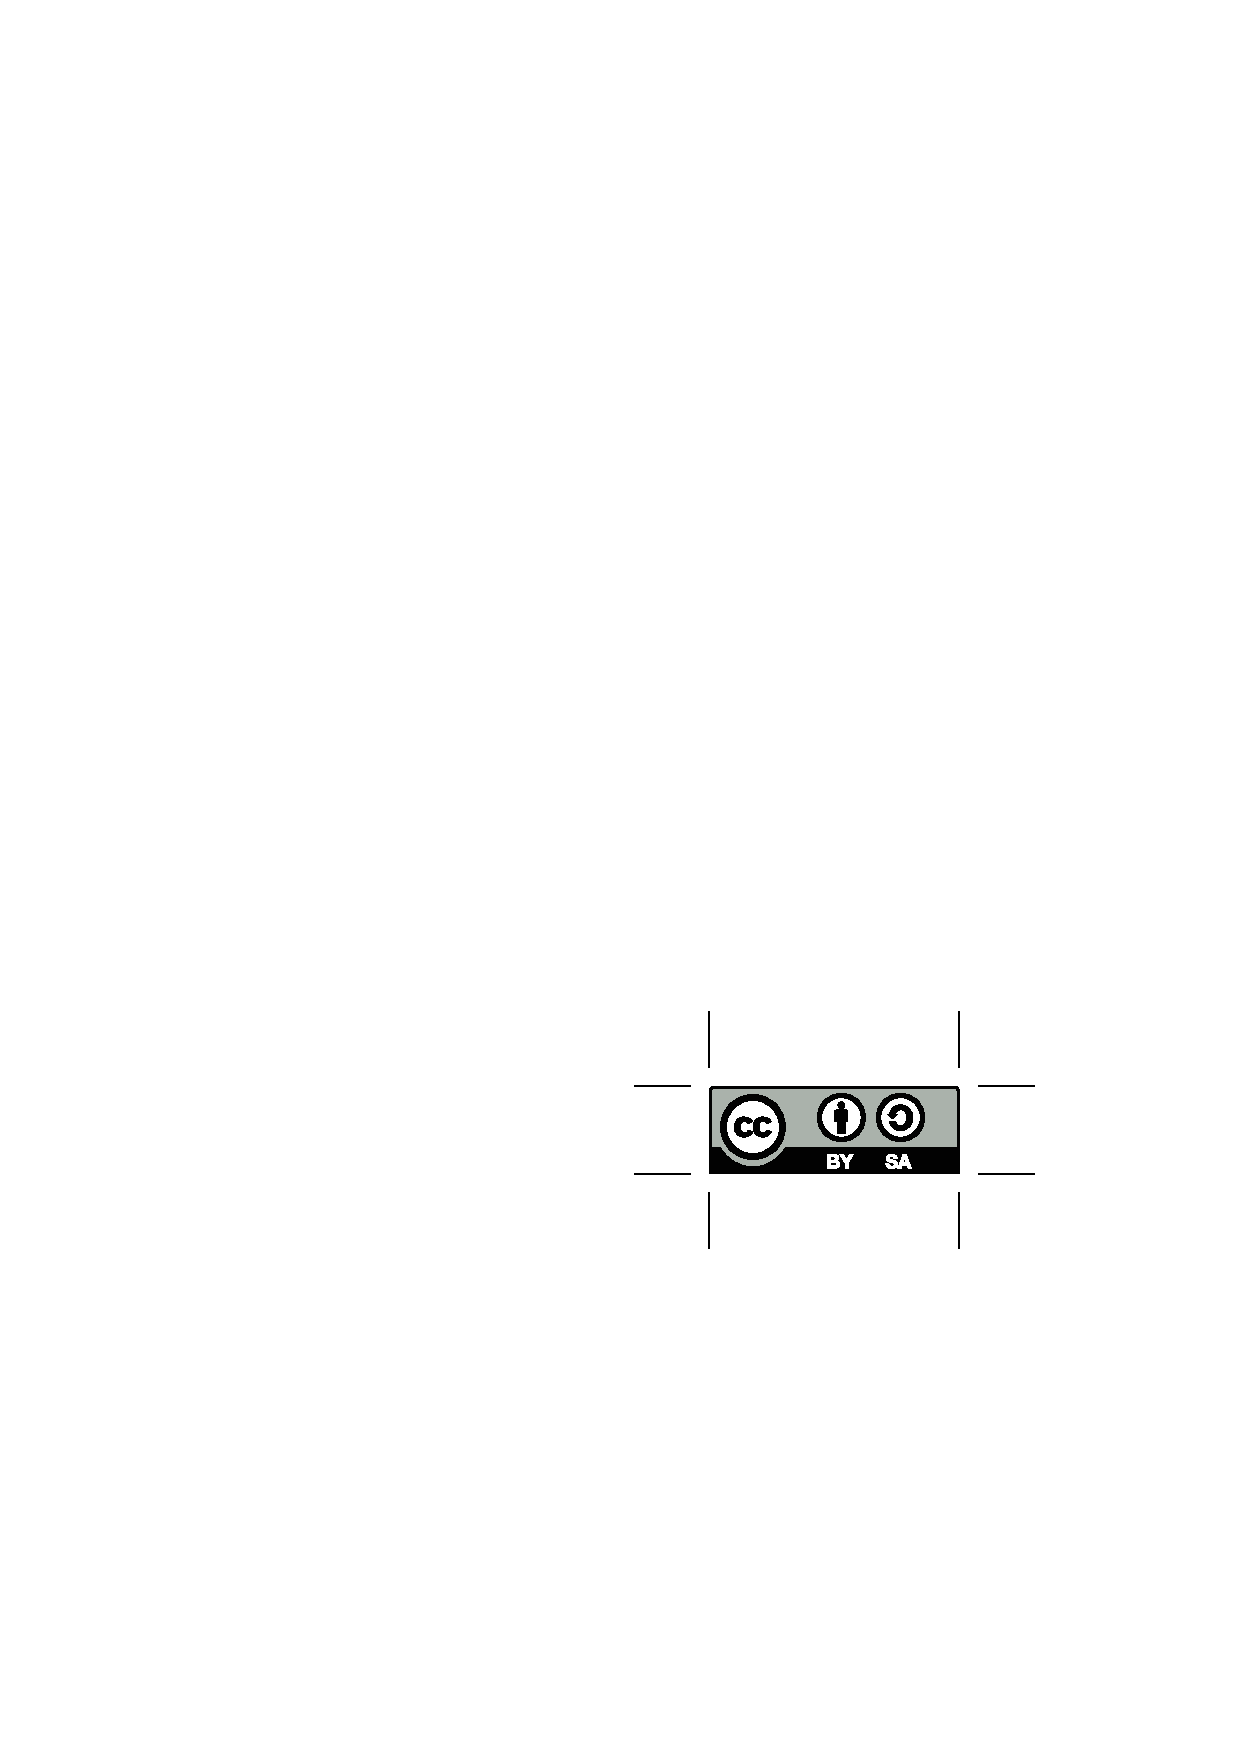
\includegraphics[width=.40\linewidth]{images/cc_by_sa}}
    \end{center}
\end{frame}

\end{document}
